\exo \textit{[Représenter]}

Voici le tableau de variations d'une fonction $f$ définie sur l'intervalle $[-1~;~3]$.

\begin{center}
\begin{tikzpicture}
 \tkzTabInit{$x$ /1 , Variations de \\$f$ /2}{$-1$, $0$, $1$, $3$}
 \tkzTabVar{-/$0$, +/$4$, -/$-6$, +/$1$}
  \end{tikzpicture}
\end{center}

\begin{enumerate}
\item Quel est le maximum de la fonction $f$ sur $[-1~;~3]$? Pour quelle valeur de $x$ est-il atteint?
\item Quel est le minimum de la fonction $f$ sur $[-1~;~3]$? Pour quelle valeur de $x$ est-il atteint?
\item Recopier et compléter l'encadrement de $f(x)$:

\og Pour tout $x \in [-1~;~3]$, $f(\ldots)\leqslant f(x) \leqslant f(\ldots)$ \fg{}. 
\end{enumerate}

\exo \textit{[Raisonner]}

\smallskip

Voici le tableau de variations d'une fonction $h$ définie sur l'intervalle $[-5~;~5]$.

\begin{center}
\begin{tikzpicture}
 \tkzTabInit{$x$ /1 , Variations de \\$h$ /2}{$-5$, $0$, $3$, $5$}
 \tkzTabVar{+/$4$, -/$-2$, +/$0$, -/$-1$}
 \tkzTabVal{1}{2}{0.5}{$-2$}{0} 
 \end{tikzpicture}
\end{center}

\smallskip

\begin{enumerate}
\item Décrire les variations de la fonction $h$ sur son ensemble de définition.
\item Comparer $h(-4)$ et $h(-3)$.  Justifier.
\item Comparer $h(1)$ et $h(2)$.  Justifier.
\item Comparer $h(3,45)$ et $h(3,6)$.  Justifier.
\item \begin{enumerate}[label=\alph*)]
\item Quel est le signe de $h(-4)$? $h(4)$?
\item Comparer alors $h(-4)$ et $h(4)$.
\end{enumerate}
\end{enumerate}

\exo \textit{[Raisonner]}
\smallskip

Voici le tableau de variations d'une fonction $f$ définie sur l'intervalle $[-2~;~5]$.

\begin{center}
\begin{tikzpicture}
 \tkzTabInit{$x$ /1 , Variations de \\$f$ /2}{$-2$, $0$, $3$, $5$}
 \tkzTabVar{+/$3$, -/$-1$, +/$2$, -/$1$}
 \tkzTabVal{1}{2}{0.5}{$-1$}{0} 
 \tkzTabVal{2}{3}{0.5}{$2$}{0} 
 \end{tikzpicture}
\end{center}

\begin{enumerate}
\item Quel est le signe de $f(x)$ lorsque $x$ appartient à l'intervalle $[-2~;~-1]$?
\item Déterminer les nombres réels $x$ de l'intervalle  $[-1~;~5]$ tels que $f(x) \geqslant 0$.
\item En déduire le tableau de signes de $f(x)$.
\end{enumerate}





\exo \textit{[Représenter]}

Soit g une fonction définie sur l’intervalle [$-8~;~4$].
\begin{itemize}[label=\ding{72},leftmargin=2cm]
\item Elle est strictement croissante sur les intervalles [$0 ;1$] et [$2 ;4$].
\item Elle est strictement décroissante sur les intervalles [$-8 ;0$] et [$1 ;2$].
\item $g(4) = 3$.
\item L’image de $-8$ est $3$ par $g$.
\item $g(0) = -1$.
\item Les antécédents de $0$ par $g$ sont $-1$ ; $0,5$ et $2$.
\item La fonction $g$ atteint son maximum pour $x = 1$. Ce maximum est $4$.
\end{itemize}

\begin{enumerate}[label=\arabic*.]
\item  Dresser le tableau de variations de la fonction $g$.
\item  Dresser le tableau de signes de $g(x)$.
\item  Tracer une courbe susceptible de représenter la fonction $g$. 
\end{enumerate}

\exo \textit{[Représenter]}

Tracer une courbe susceptible de représenter graphiquement la fonction $f$ de l'exercice 2 de cette fiche.

\exo

$f$ est la fonction définie sur [$1~;~5$] par:

\[f(x)=x+\dfrac{4}{x}\]

\begin{enumerate}
\item Afficher la courbe représentative de la fonction $f$ à l'écran de votre calculatrice.
\item Indiquer les réglages utilisés pour la fenêtre.
\item Conjecturer le sens de variation de la fonction $f$.
\end{enumerate}

\exo \textit{[Représenter]}

$f$ est la fonction définie sur $\R$ par:

\[f(x)=x^2-2x+2\]

Clément dit : \og J'ai trouvé $f(0)=2$ et $f(3)=5$, donc $f$ est croissante sur [$0~;~3$] \fg{} . Qu'en pensez-vous?

\exo \textit{[Chercher]}

Parmi les expressions suivantes, lesquelles définissent une fonction affine? Justifier la réponse.

a) $f(x)=-4x$ \hspace{0.9 cm} b) $g(x)=\dfrac{x-2}{4}$ \hspace{0.8 cm} c) $h(x)=\sqrt{2}x-1$ 

d) $i(x)=\dfrac{x-3}{x}$ \hspace{0.8 cm} e) $j(x)=2$ \hspace{1.6 cm} f) $k(x)=2x^2-1$ 

\exo \textit{[Modéliser, Calculer]}

Un hypermarché propose $12$~\% de réduction sur tous les produits de la marque propre au magasin pour les détenteurs de la carte fidélité du magasin. 

\begin{enumerate}
\item Un article de la marque propre au magasin est affiché au prix de 15 \euro. Quelle sera le prix après la réduction consentie?
\item Voici un algorithme qui affiche le prix d'un article après la réduction de $12$~\%.

\begin{tabular}{|p{10cm}}
p=float(input(" Entrer le prix de l'article "))\\
$p_{final}$= \ldots  \\
print($p_{final}$)\\
\end{tabular}

\medskip

Compléter l'algorithme.

\item Écrire une fonction nommée \og $prix$ \fg{}  qui renvoie le prix d'un article après la réduction.

\item R est la fonction qui au prix $x$ (en \euro) d'un article associe le prix (en \euro) après réduction.

\begin{enumerate}[label=\alph*)]
\item Donner l'expression de $R(x)$ en fonction de $x$.
\item Quelle est la nature de la fonction $R$?
\end{enumerate}
\end{enumerate}

\exo \textit{[Calculer]}

\begin{enumerate}
\item Dans chaque cas $f$ est une fonction affine de taux d'accroissement $a$. Calculer :

\begin{enumerate}[label=\alph*)]
\item $f(7)-f(3)$ lorsque $a=5$. 
\item $f(2025)-f(2024)$ lorsque $a=-\dfrac{13}{7}$.
\item $f(2)-f(-1)$ lorsque $a=2.5$.
\end{enumerate}

\item $g$ est une fonction affine définie par $g(x)=5-3x$.

Calculer $g(-11)-g(-13)$ de deux façons différentes.
\end{enumerate}


\exo \textit{[Chercher, calculer]}

\begin{enumerate}
\item Une fonction affine $f$ est telle  que $f(3)=10$ et $f(6)=4$.
\begin{enumerate}[label=\alph*)]
\item Montrer que le taux d'accroissement $a$ de la fonction $f$ est égal à $-2$.
\item  En utilisant $f(3)=10$, montrer que : $-6+b=10$.
\item En déduire $b$ et l'expression de la fonction affine $f$.
\end{enumerate}
\item Trouver, de la même façon, l'expression de la fonction affine $f$ telle que $f(2)=-5$ et $f(7)=10$.
\end{enumerate}


\exo \textit{[Raisonner]}

Donner le sens de variation et l'éventuelle parité des fonctions affines suivantes:

\begin{enumerate}
\item $f(x)=6x-8$.
\item $f(x)=-6x$.
\item $f(x)=8-6x$.
\item $f(x)=8$.
\end{enumerate}

\exo \textit{[Raisonner]}

\begin{enumerate}
\item Si $x_1<x_2$ alors on souhaite comparer : $\dfrac{1}{2}x_1-1$ et $\dfrac{1}{2}x_2-1$.

Compléter:
La fonction affine $f$, impliquée est définie par  $f(x)=..........................................$.

Puisque $a=...............$, $f$ est strictement ............................ sur $\R$ et l'ordre des images est .................................. par rapport à celui des antécédents.

Donc \og Si $x_1<x_2$ alors $f(\ldots) \ldots f(\ldots $ d'où $\dfrac{1}{2}x_1-1$ ..............................................................\fg{} .


\item Dans chaque cas, suivre un raisonnement analogue afin de compléter les propriétés.

\begin{enumerate}[label=\alph*)]
\item \og Si $x_1<x_2$ alors $-2x_1+3$ ... $-2x_2+3$ \fg{}.
\item \og Si $x_1<x_2$ alors $\dfrac{x_1}{3}$ ... $\dfrac{x_2}{3}$ \fg{}.
\item \og Si $x_1>x_2$ alors $x_1+2025$ ... $x_2+2025$ \fg{}.
\end{enumerate}
\end{enumerate}

\exo \textit{[Raisonner]}

\begin{enumerate}
\item $x$ et $y$ désignent deux nombres réels tels que: $-2<x<6$ et $1<y<4$. Justifier les inégalités suivantes :
\begin{enumerate}[label=\alph*)]
\item $-1<x+y<10$
\item $-4<-y<-1$
\item $-6<x-y<5$
\end{enumerate}
\item Soient deux nombres réels $x$ et$y$ tels que $x \leqslant 2$ et $y \leqslant 6$. Que peut-on dire des expressions suivantes ?
\begin{enumerate}[label=\alph*)]
\item $3x$
\item $-4y$
\item $x-5$
\item $x+y$
\end{enumerate}

\end{enumerate}




      

